\documentclass{book} % Definisi jenis dokumen

%%%%% Definisi paket-paket yang seharusnya digunakan %%%%%
\usepackage[utf8]{inputenc} % paket encoding input utf8
\usepackage[T1]{fontenc} % paket encoding huruf latin
\usepackage{tocbibind} % paket toc terdaftar dalam toc

%%%%% Definisi paket-paket yang digunakan sesuai kebutuhan %%%%%
\usepackage[yyyymmdd,hhmmss]{datetime} % paket tanggal-waktu
\usepackage{geometry} % paket ukuran kertas dan margin
\usepackage{graphicx} % paket grafik/gambar
\usepackage{subcaption} % paket untuk subfigure
\usepackage{minted} % paket untuk source code
\usepackage{xcolor} % paket buat warna
\usepackage{hyperref} % paket buat link-link an
\usepackage{minted} % paket lingkungan kode sumber

%%%%% Pengaturan ukuran kertas dan margin %%%%%
\geometry{
	a4paper,
	left=10mm,
	right=10mm,
	top=15mm,
	bottom=15mm,
}

%%%%% Pengaturan perintah informasi perangkat lunak (hanya untuk GNU/Linux) %%%%%
\newcommand{\ShowOsVersion}{
	\immediate\write18{\unexpanded{foo=`uname -sro` && echo "${foo}" > tmp.tex}}
	\input{tmp}\immediate\write18{rm tmp.tex}
}

\newcommand{\ShowTexVersion}{
	\immediate\write18{\unexpanded{foo=`pdflatex -version | head -n1 | cut -d' ' -f1,2` && echo "${foo}" > tmp.tex}}
	\input{tmp}\immediate\write18{rm tmp.tex}
}

\definecolor{LightGray}{gray}{0.95}

\hypersetup{
	colorlinks=true, %set true if you want colored links
	linktoc=all,     %set to all if you want both sections and subsections linked
	linkcolor=blue,  %choose some color if you want links to stand out
	urlcolor=blue,   %url color
}

\begin{document}
	%%%%%%%%%%%%%%%%%%%%%%%%%%%%%%%%%%%%%%%%%%%%%%%%%%%%%%%%%%%%%%%%%
	
	\frontmatter % untuk halaman cover
	
	\begin{titlepage}
		
		\centering % untuk membuat tengah teks
		
		{
			\LARGE % pakai font besar
			\bf % pakai font BOLD
			Rangkuman Kegiatan Pengembangan Telemetri Vibrasi
		}
		
		\bigskip
		{\Large \bf Achmadi ST MT}
		\vfill % menambahkan ruang kosong vertikal
		
		\includegraphics[width=300pt]{images/vibslogo}
		\vfill
		
		\raggedright
		\noindent Dokumen ini ditulis dengan:\\ % tanda \\ menambahkan garis baru
		OS : \ShowOsVersion \\
		TeX : \ShowTexVersion \\
		Update: {\today} at \currenttime\\
	\end{titlepage}
	
	%%%%%%%%%%%%%%%%%%%%%%%%%%%%%%%%%%%%%%%%%%%%%%%%%%%%%%%%%%%%%%%%%
	
	\newpage % halaman baru
	\tableofcontents % daftar isi
	\listoffigures % daftar gambar
	\listoftables % daftar table
	
	%%%%%%%%%%%%%%%%%%%%%%%%%%%%%%%%%%%%%%%%%%%%%%%%%%%%%%%%%%%%%%%%%
	
	\mainmatter % pindah format halaman dari romawi ke angka (konten utama)
	
	\newpage
	\chapter{Goal}
	
	\section{Diagram Sistem}
	
	Berikut rangkuman tujuan akhir pengembangan:
	
	\begin{figure}[!ht]
		\centering
		\includegraphics[width=0.8\textwidth]{images/goal_diagram/goal}
		\caption{Diagram Pembangunan Sistem Monitoring}
	\end{figure}
	
	\section{Pemilihan Komponen}
	
	\subsection{Sensor Vibrasi}
	
	Sensor Vibrasi menggunakan TE-850M1:
	
	\begin{itemize}
		\item Analog Output 
		\item VDD Level Voltage (3.3V)
		\item Triaxial on separate
		\item Up to 25G vibration
	\end{itemize}
	
	\newpage
	\subsection{Microcontroller}
	
	Microcontroller menggunakan seri STM32Fx LQFP64:
	
	\begin{itemize}
		\item Arsitektur ARM Cortex-M
		\item VDD Level Voltage (3.3V)
		\item PLL hingga 72MHz
		\item ADC hingga 12bit
		\item Memiliki mode sleep dengan konsumsi rendah
		\item Harga terjangkau
	\end{itemize}
	
	\subsection{Transceiver}
	
	Module Radio Transceiver menggunakan seri LoRA SX1278:
	
	\begin{itemize}
		\item VDD Level Voltage (3.3V)
		\item Konsumsi daya rendah
		\item Frekuensi 433MHz (Kategori Pita 31 menurut UU Kominfo Tahun 2018)
		\item Termasuk non-3GPP sehingga tidak overlap dengan jaringan selular.
		\item Dapat menjangkau area hingga radius 10km (RSSI minimal)
		\item Harga terjangkau
	\end{itemize}
	
	\newpage
	\chapter{Development Stages}
	
	\section{Sensor Testing}
	
	Tahapan ini bertujuan untuk menguji antar muka sensor vibrasi TE-850M1 ke STM32.
	
	\subsection{Setup Pengujian}
	
	\begin{figure}[!ht]
		\centering
		\begin{subfigure}{0.3\textwidth}
			\includegraphics[width=\textwidth]{images/vibparts.png}
			\caption{Mockup}
		\end{subfigure}
		\begin{subfigure}{0.3\textwidth}
			\includegraphics[width=\textwidth]{images/vibs.png}
			\caption{Actual}
		\end{subfigure}
		\caption{Preview Unit}
	\end{figure}
	
	\begin{figure}[!ht]
		\centering
		\includegraphics[width=0.6\textwidth]{images/testing}
		\caption{Diagram Pengujian}
	\end{figure}
	
	\newpage
	\begin{figure}[!ht]
		\centering
		\includegraphics[width=0.65\textwidth]{images/testactual.jpg}
		\caption{Dokumentasi Testing}
	\end{figure}
	
	\subsection{Desain Purwarupa}
	
	\begin{itemize}
		\item Skematik: \href{https://github.com/VibrasticLab/wesel_monitoring/blob/master/circuit/mems_vibs/mems_vibs.kicad_sch}{Github}
		
		\begin{figure}[!ht]
			\centering
			\includegraphics[width=\textwidth]{images/mems_vibs-sch.png}
			\caption{Skematik}
		\end{figure}
		
		\newpage
		\item Layout: \href{https://github.com/VibrasticLab/wesel_monitoring/blob/master/circuit/mems_vibs/mems_vibs.kicad_pcb}{Github}
		
		\begin{figure}[!ht]
			\centering
			\includegraphics[width=\textwidth]{images/mems_vibs-brd.png}
			\caption{Layout PCB}
		\end{figure}
	
		\item Code Snippet untuk sampling ADC dengan sampling interval setiap 125uS dan print out ke Serial UART.\\
		Source: \href{https://github.com/VibrasticLab/wesel_monitoring/blob/master/firmware/vib/vib_analog.c#L42-L64}{Github}

		\begin{minted}[frame=lines,framesep=2mm,fontsize=\normalsize,bgcolor=LightGray]{c}
if(adcp->state == ADC_COMPLETE){
	sum_adc_tps = 0;
	
	for(i=0;i<ADC_GRP1_BUF_DEPTH;i++){
		sum_adc_tps = sum_adc_tps + samples[0 + (i*ADC_GRP1_NUM_CHANNELS)];
	}
	
	adc_z = sum_adc_tps/10;
	
	chprintf((BaseSequentialStream*)&SD1,"%4i\r\n",adc_z);
}
		\end{minted}
		
		\begin{minted}[frame=lines,framesep=2mm,fontsize=\normalsize,bgcolor=LightGray]{c}
static THD_WORKING_AREA(wa_adcThread, 128);
static THD_FUNCTION(adcThread, arg) {
	(void)arg;
	while (TRUE) {
		chThdSleepMicroseconds(125);
		adcStartConversion(&ADCD1, &adcgrpcfg, samples, ADC_GRP1_BUF_DEPTH);
	}
}
		\end{minted}
		
		\begin{minted}[frame=lines,framesep=2mm,fontsize=\normalsize,bgcolor=LightGray]{c}
palSetPadMode(GPIOA, 0, PAL_MODE_INPUT_ANALOG);

adcStart(&ADCD1, NULL);
chThdCreateStatic(wa_adcThread, sizeof(wa_adcThread), NORMALPRIO, adcThread, NULL);

palSetPadMode(GPIOA, 9, PAL_MODE_STM32_ALTERNATE_PUSHPULL);
palSetPadMode(GPIOA, 10, PAL_MODE_INPUT);

sdStart(&SD1, NULL);
		\end{minted}

	\newpage
	
	\item Code Snippet untuk Interface untuk menerima data plot di komputer via serial USB.\\
	Source: \href{https://github.com/VibrasticLab/wesel_monitoring/blob/master/interface/python/plot_test/serialplot.py}{Github} 
	
	\begin{figure}[!ht]
		\centering
		\includegraphics[width=\textwidth]{images/protoiface.png}
		\caption{Interface}
	\end{figure}
	\end{itemize}
	
	\begin{minted}[frame=lines,framesep=2mm,fontsize=\normalsize,bgcolor=LightGray]{c}
self.canvas = FigureCanvasTkAgg(self.fig, master=self.graphfrm)
self.canvas.draw()
self.canvas.get_tk_widget().pack(side=tk.LEFT)

self.serPort = serial.Serial(port=sys.argv[1],baudrate=115200,timeout=0)

self.aniplot = plotani.FuncAnimation(self.fig, self.graphupdate, interval=0.00005, repeat=False, cache_frame_data=False)
self.aniplot._start()

self.serThd = thd(target=self.serial_read).start()
	\end{minted}
	
	\begin{minted}[frame=lines,framesep=2mm,fontsize=\normalsize,bgcolor=LightGray]{c}
 def serial_read(self):
	while self.SerThdRun:
	serVal = self.serPort.readline()
	if len(serVal)>5: # %4i and CR/LF
	valY = int(serVal)
	self.array_value(valY)
	
	sleep(0.0001)
	\end{minted}
	
	\newpage
	\section{Radio Testing}
	
	Tahapan ini bertujuan untuk menguji modul radio SX1278 dan antar muka ke chip STM32.
	
	\subsection{Setup Pengujian}
	
	\begin{figure}[!ht]
		\centering
		\includegraphics[width=0.6\textwidth]{images/lora/tesLora.png}
		\caption{Diagram Pengujian LoRa}
	\end{figure}
	
	\begin{figure}[!ht]
		\centering
		\includegraphics[width=0.5\textwidth,angle=180]{images/lorates.jpg}
		\caption{Setup Pengujian LoRa}
	\end{figure}
	
	\newpage
	
	Hasil pengembangan:
	
	\begin{figure}[!ht]
		\centering
		\begin{subfigure}{0.4\textwidth}
			\includegraphics[width=\textwidth]{images/lorasend.png}
			\caption{Transmitter}
		\end{subfigure}
		\begin{subfigure}{0.4\textwidth}
			\includegraphics[width=\textwidth]{images/lorareceiv.png}
			\caption{Receiver}
		\end{subfigure}
		\caption{Testing Komunikasi}
	\end{figure}
	
	Dikembangkan pustaka LoRa via SPI untuk abstraksi ChibiOS/RT pada target chip STM32: \href{https://github.com/mekatronik-achmadi/example_collection/tree/master/embedded/stm32/bluepill_lora/lora}{Github}.
	
	\begin{minted}[frame=lines,framesep=2mm,fontsize=\normalsize,bgcolor=LightGray]{c}
static const SPIConfig spicfg = {
	NULL,
	GPIOA,
	LORA_DEFAULT_NSS_PIN,
	0
};
	\end{minted}
	
	\begin{minted}[frame=lines,framesep=2mm,fontsize=\normalsize,bgcolor=LightGray]{c}
static uint8_t lora_singleTransfer(uint8_t address, uint8_t value){
	uint8_t txbuf[1], rxbuf[1];
	
	txbuf[0] = value;
	
	palClearPad(GPIOA, LORA_DEFAULT_NSS_PIN);
	
	spiSelect(&SPID1);
	spiSend(&SPID1, sizeof(address), &address);
	spiExchange(&SPID1, sizeof(txbuf), txbuf, rxbuf);
	spiUnselect(&SPID1);
	
	palSetPad(GPIOA, LORA_DEFAULT_NSS_PIN);
	
	return rxbuf[0];
}
	\end{minted}
	
	\newpage
	\section{Pengembangan Selanjutnya}
	
	\subsection{Desain}
	
	\begin{itemize}
		\item Skematik: \href{https://github.com/VibrasticLab/wesel_monitoring/blob/master/circuit/mems_lora/mems_lora.kicad_sch}{Github}
	
		\begin{figure}[!ht]
			\centering
			\includegraphics[width=\textwidth]{images/mems_lora-sch.png}
			\caption{Skematik}
		\end{figure}
		
		\item PCB: \href{https://github.com/VibrasticLab/wesel_monitoring/blob/master/circuit/mems_lora/mems_lora.kicad_pcb}{Github}
		
		\begin{figure}[!ht]
			\centering
			\includegraphics[width=\textwidth]{images/mems_lora-brd.png}
			\caption{PCB}
		\end{figure}
		
		\newpage
		\item MockUp Unit
		
		\begin{figure}[!ht]
			\centering
			\includegraphics[width=0.6\textwidth]{images/mems_lora.png}
			\caption{Mockup Unit}
		\end{figure}
		
		\item MockUp Casing
		
		\begin{figure}[!ht]
			\centering
			\includegraphics[width=0.8\textwidth]{images/casingpov.png}
			\caption{Mockup Casing}
		\end{figure}
	
	\end{itemize}
\end{document}